%projets
Lors de ce sprint , nous allons raffiner le cas d’utilisation "gestion du projet" .
D\'{e}tailler le cas d'utilisation \guillemotleft{} "Gestion du projet " \guillemotright{} revient \`{a} d\'{e}tailler
ses sous cas d'utilisation \`{a} savoir :
\textbullet{} Gestion des t\^{a}ches.
\textbullet{} Gestion des projets
\subsubsection{Analyse}

\subsubsection{ Diagramme de cas d'utilisation "G\'{e}rer un projet"}

\begin{figure}[H]
\center
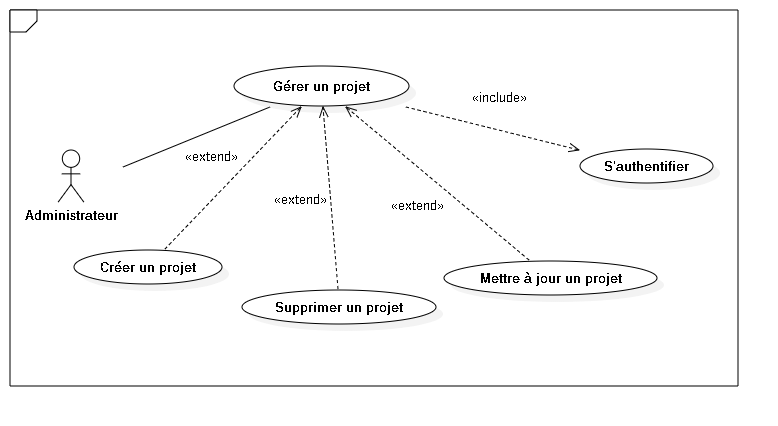
\includegraphics[width=13cm,height=8cm]{./figures/ucP.png}
\caption{G\'{e}rer un projet.}

\end{figure}

\subsubsection{ Diagramme de cas d'utilisation "G\'{e}rer une t\^{a}che"}
\begin{figure}[H]
\center
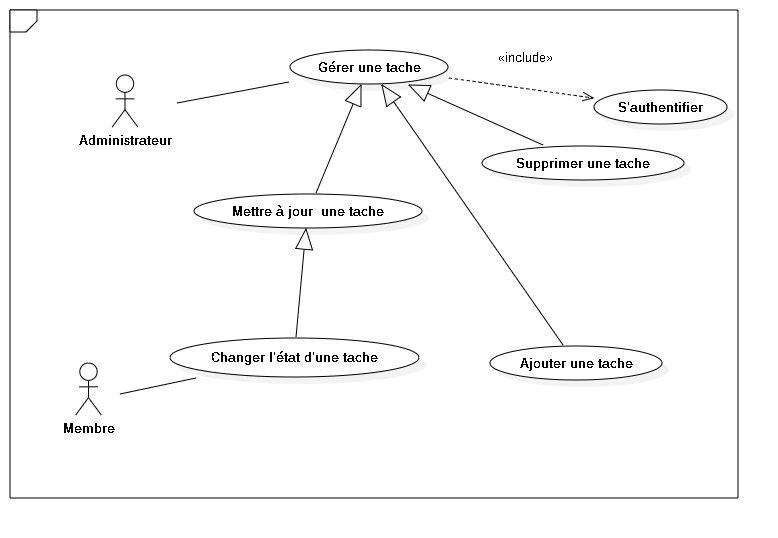
\includegraphics[width=13cm,height=8cm]{./figures/ucT.png}
\caption{G\'{e}rer une t\^{a}che.}

\end{figure}



\subsubsection{Conception}
\subsubsection{  Le sc\'{e}nario \guillemotleft{} Cr\'{e}ation d'un projet \guillemotright{}}

Le diagramme de s\'{e}quence \guillemotleft{} Ajout d'un projet \guillemotright{} pr\'{e}sente un s\'{e}quencement
des interactions entre Administrateur, Application et Base de donn\'{e}es (BD) .


\begin{figure}[H]
\center
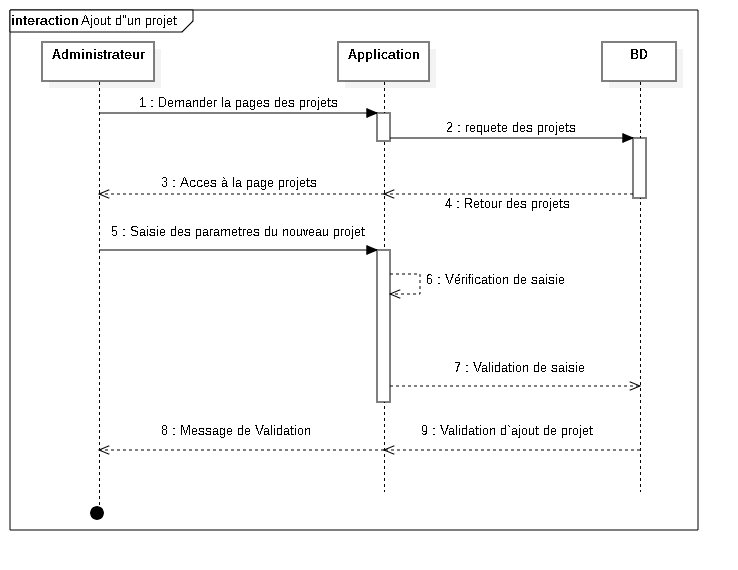
\includegraphics[width=14cm,height=11cm]{./figures/seq/B.png}
\caption{ Cr\'{e}ation d'un projet.}
\end{figure}

\newpage
\subsubsection{Le sc\'{e}nario \guillemotleft{} Cr\'{e}ation d'une t\^{a}che\guillemotright{}}
Le diagramme de s\'{e}quence \guillemotleft{} Ajout d'une t\^{a}che \guillemotright{} pr\'{e}sente le s\'{e}quencement
des interactions entre Administrateur, Application et Base de donn\'{e}es (BD).

\begin{figure}[H]
\center
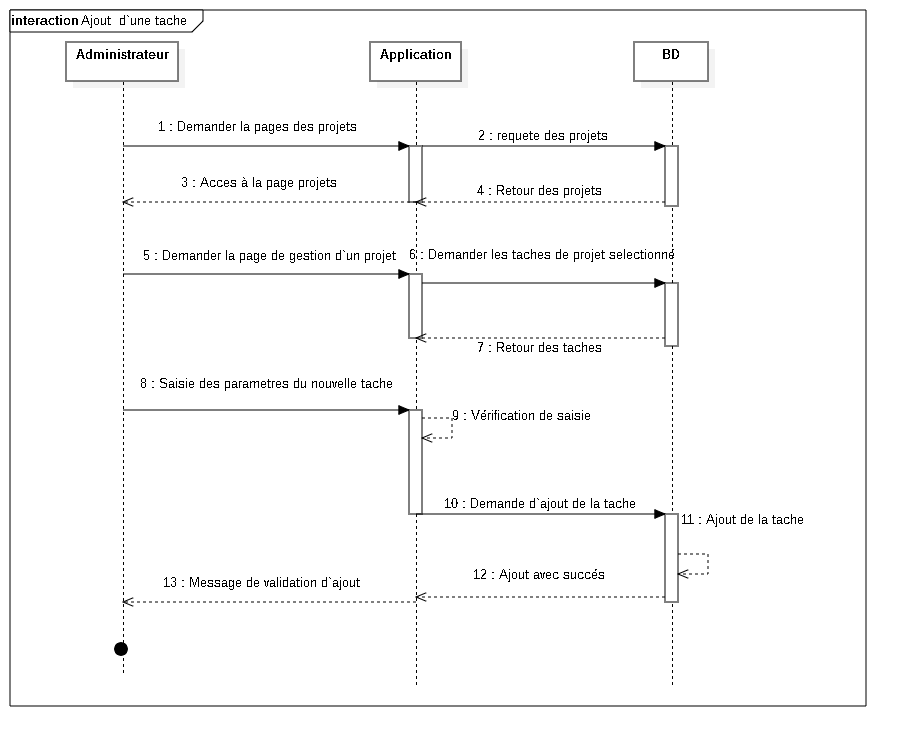
\includegraphics[width=14cm,height=13cm]{./figures/seq/C.png}
\caption{Cr\'{e}ation d'une t\^{a}che.}
\end{figure}





\subsubsection{Sch\'{e}mas}
\FloatBarrier

\begin{table}

\begin{tabular}{|l|l|l|l|l|l|}
\hline
Field         & Type          & Null & Key & Default & Extra            \\
\hline
id            & int(11)       & NO   & PRI & NULL    & auto\_increment  \\
\hline
name          & varchar(45)   & NO   &     & NULL    &                  \\
\hline
description   & varchar(1000) & YES  &     & NULL    &                  \\
\hline
start         & date          & NO   &     & NULL    &                  \\
\hline
end           & date          & NO   &     & NULL    &                  \\
\hline
category      & varchar(60)   & YES  &     & NULL    &                  \\
\hline
customers\_id & int(11)       & YES  & MUL & NULL    &                  \\
\hline
\end{tabular}
\centering
 \caption {Projects.}
\end{table}
\FloatBarrier

\subsubsection{Test}
C'est l'interface principale de notre application
\FloatBarrier
\begin{figure}[H]
\center
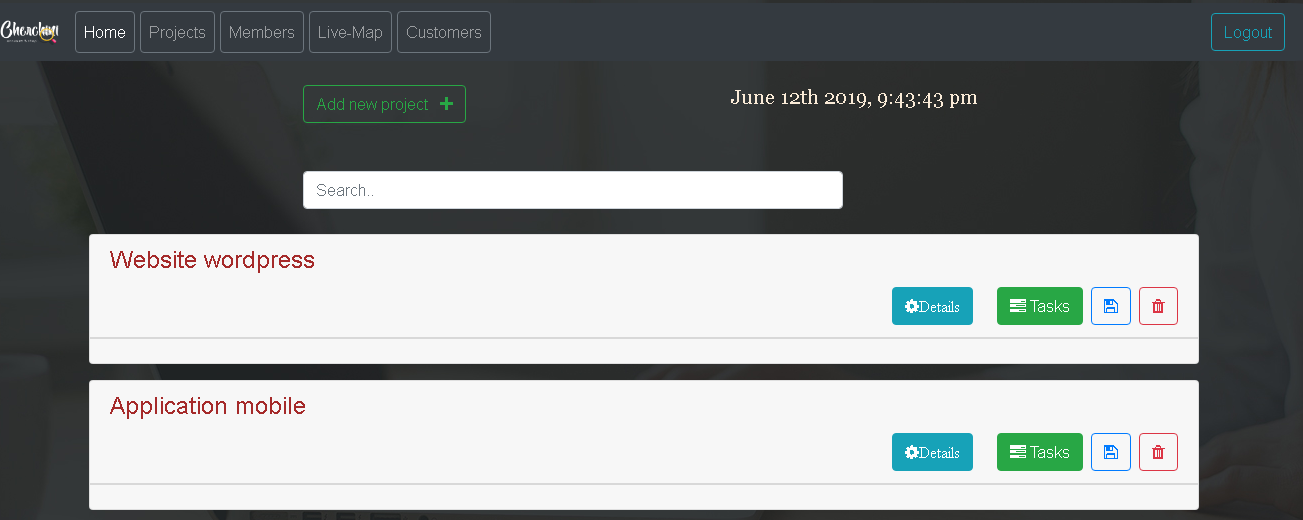
\includegraphics[width=11cm,height=7cm]{./figures/pres/gp1.png}
\caption{Gestion de projet.1.}
\end{figure}
\FloatBarrier

Nous ajoutons un nouveau projet et l'assignons un ou plusieurs membres.
\FloatBarrier
\begin{figure}[H]
\center
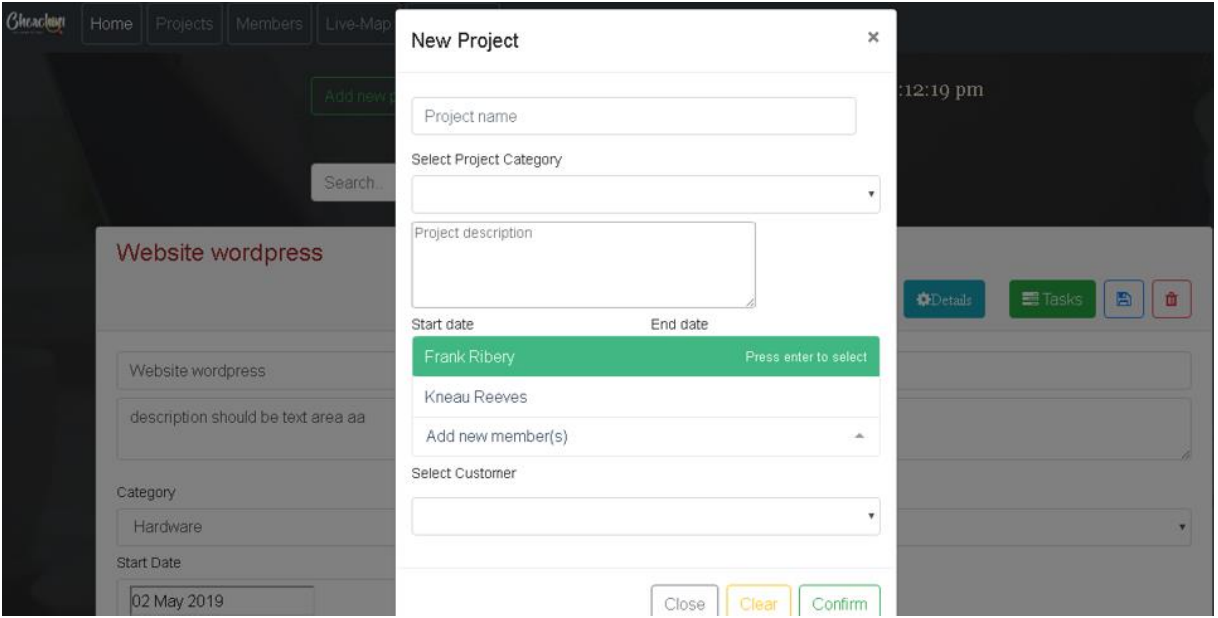
\includegraphics[width=11cm,height=7cm]{./figures/pres/gp2.png}
\caption{Gestion de projet.2.}
\end{figure}
\FloatBarrier

\FloatBarrier
\begin{figure}[H]
\center
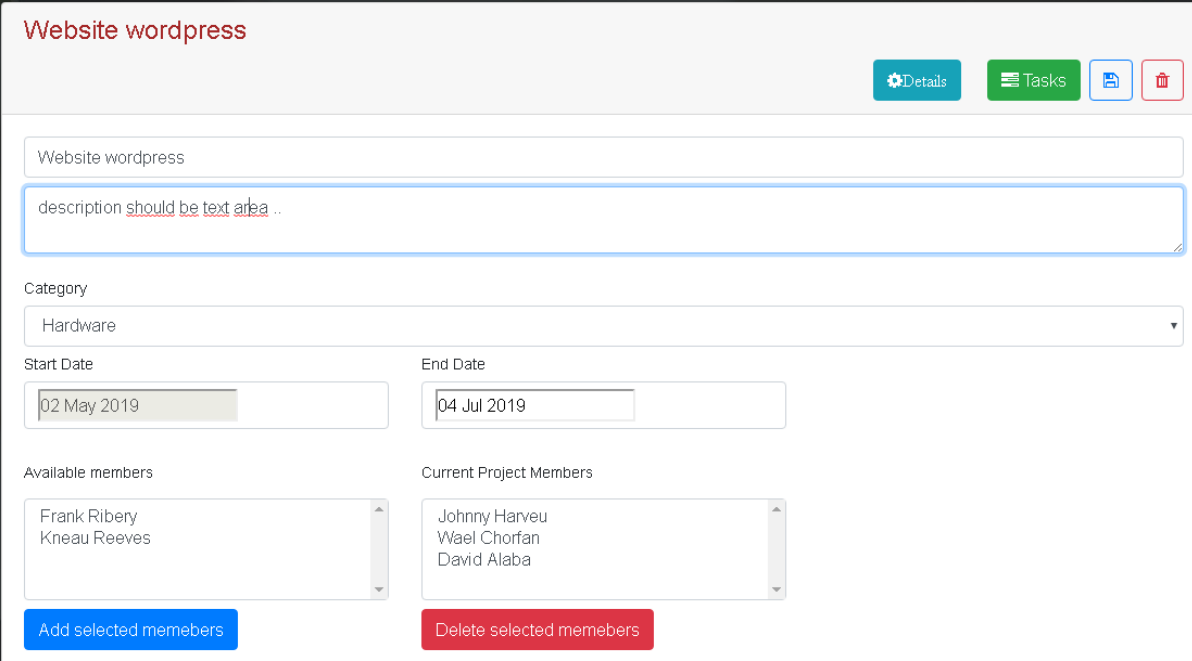
\includegraphics[width=11cm,height=7cm]{./figures/pres/gp3.png}
\caption{Gestion de projet.3.}
\end{figure}
\FloatBarrier

Pour chaque projet en cliquant sur le buttons Details ,on peut modifier ses
d\'{e}tails ,on peut s\'{e}l\'{e}ectionner plusieurs membres et les ajouter .
On ne peut pas modifier les dates de d\'{e}but et de fin puisque les dates des
taches devraient etre p\'{e}nibles \`{a} changer tache par tache .

\bigskip
\bigskip

En cliquant sur le button \guillemotleft{} Tasks \guillemotright{} d'un certain projet , l'administrateur est
amen\'{e}e \`{a} l'interface de gestion des taches correspondantes dans laquelle il
peux suivre la progression des taches ,consulter le diagramme de gannt
dynamique et modifier les param\'{e}tres des taches .

\FloatBarrier
\begin{figure}[H]
\center
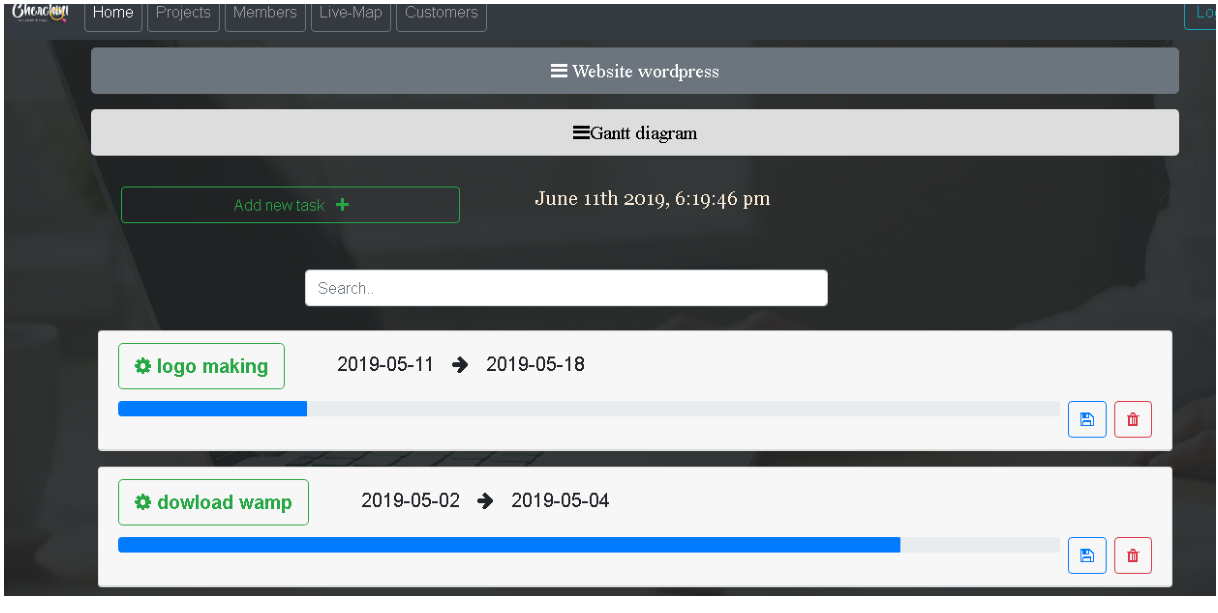
\includegraphics[width=11cm,height=7cm]{./figures/pres/gp4.png}
\caption{Gestion de projet.4.}
\end{figure}
\FloatBarrier



\FloatBarrier
\begin{figure}[H]
\center
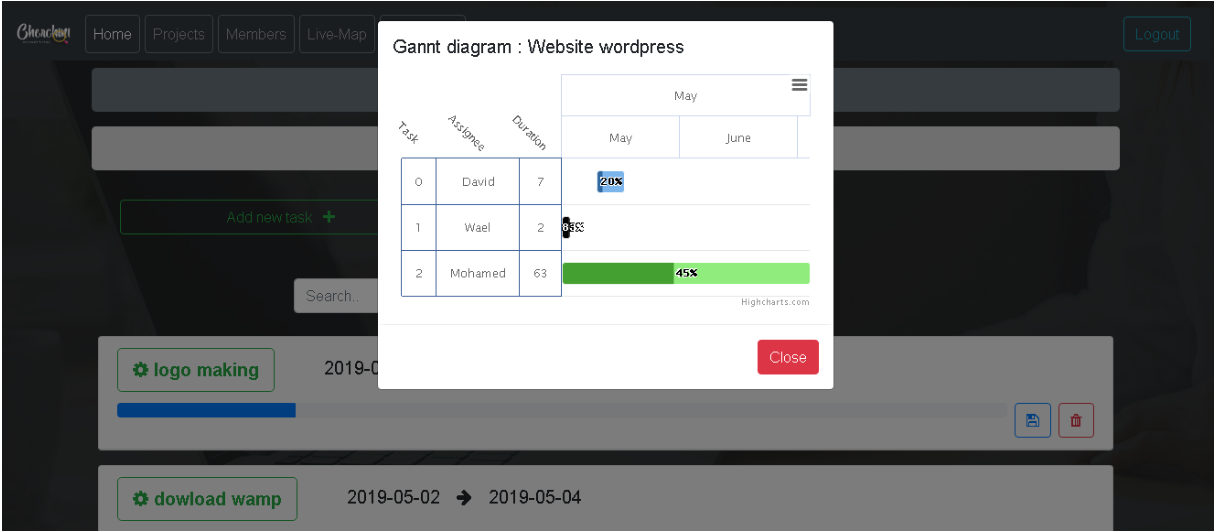
\includegraphics[width=11cm,height=7cm]{./figures/pres/gp5.png}
\caption{Gestion de projet.5.}
\end{figure}
\FloatBarrier


\FloatBarrier
\begin{figure}[H]
\center
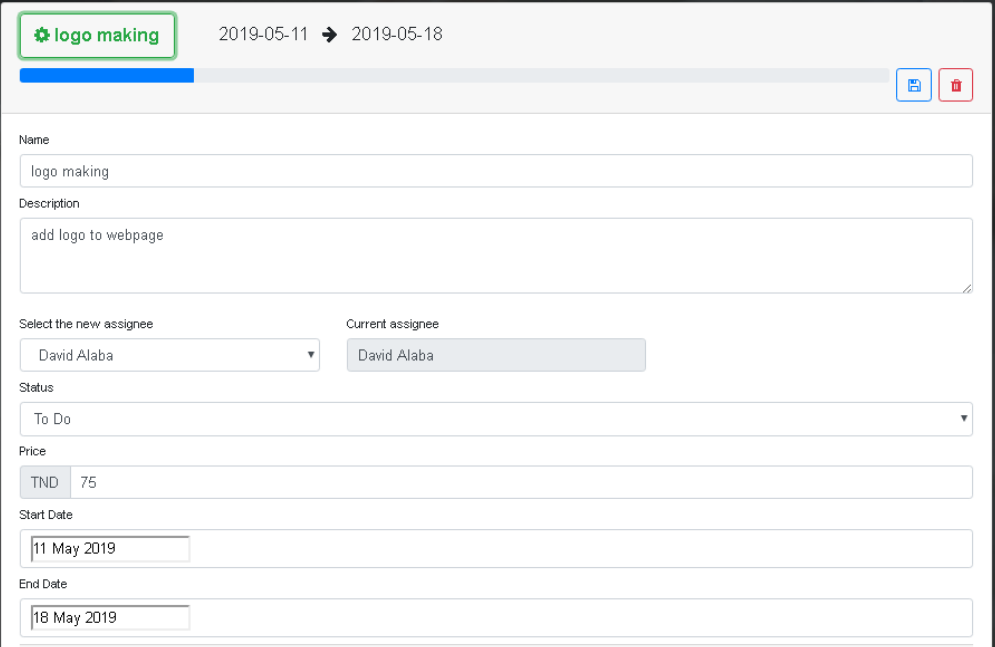
\includegraphics[width=11cm,height=7cm]{./figures/pres/gp6.png}
\caption{Gestion de projet.6.}
\end{figure}
\FloatBarrier 